\documentclass[thesis.tex]{subfiles}

\title{Estimating duration in the presence of misclassification}
\author{Joshua Blake}
\date{\today}

\begin{document}

\ifSubfilesClassLoaded{
  \setcounter{chapter}{1}
}

\chapter{SARS-CoV-2: biology and data} \label{biology-data}

\todo[inline]{Rewrite chapter 2 intro after writing thesis intro because it will be clearer how to divide content.}

SARS-CoV-2 is a beta coronavirus that emerged in late 2019.
It is closely related to previous coronaviruses that have caused outbreaks in humans, SARS-CoV and MERS-CoV.
\todo{Cite and check how SARS-CoV-2 is related to SARS-CoV and MERS-CoV, and other human coronaviruses.}

Coronaviruses are RNA (Ribonucleic acid) viruses.
RNA viruses use RNA, rather than DNA, as their genetic material.
\todo{why is being a RNA virus important?}

\section{Natural history of the disease} \label{biology-data:sec:natural-history}

\begin{figure}
  \centering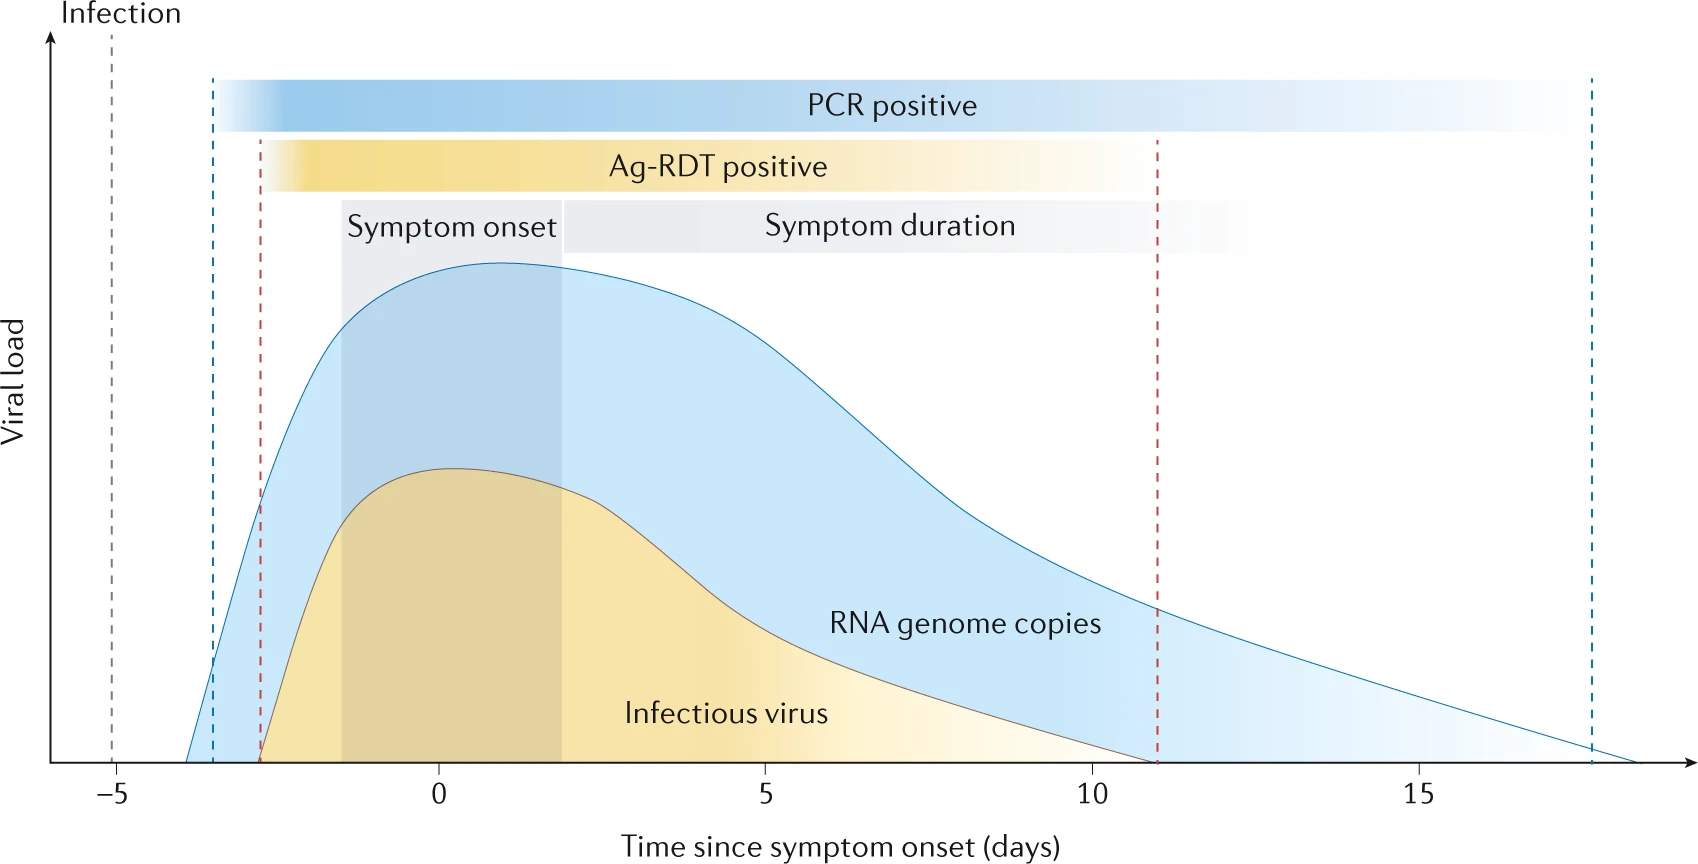
\includegraphics[width=\textwidth]{biology-data/natural-history}
  \caption[Natural history of SARS-CoV-2.]{Natural history of SARS-CoV-2. Reproduced from \textcite{puhachSARSCoV2} with permission.}
  \todo[inline]{Define the acronyms and terminology in the figure.}
  \label{biology-data:fig:natural-history}
\end{figure}

An individual infected with SARS-CoV-2 goes through several stages (see \cref{biology-data:fig:natural-history}).
\todo{Find citations for disease stages.}
First, they are exposed to the virus and become infected.
At this initial stage they are not infectious (cannot spread the disease to others), do not have symptoms, and will not test positive on a PCR test.
After a few days, they will start testing positive on a PCR test; this is normally prior to being infectious or having symptoms.
Next, the individual becomes infectious; normally, this occurs prior to symptom onset for those who experience symptoms.
Recovery from symptoms occurs after a few days, around individual is no longer infectious.
Finally, the individual will test negative on a PCR test.
\todo{Talk about PCR testing detecting RNA material even with no viable virus.}

The time for each of these stages depends on various features of host and virus characteristics.
In this thesis, I focus on pre-Alpha variants of SARS-CoV-2 in unvaccinated individuals.
The time from infection to infectiousness is known as the \emph{latent period} and is typically around\todo{cite latent period}.
The time from infection to experiencing symptoms is known as the \emph{incubation period} and is typically around\todo{cite incubation period}.
The latent period is undefined for asymptomatic individuals, around\todo{cite proportion asymptomatic} of those infected.

The above description gives three possible ways to define an individual who is infected with SARS-CoV-2: based on their PCR test result, whether they are infectious, or whether they are symptomatic.
In this thesis, I adopt a definition of infection based on PCR test results.
This is because it coincides with the data collected on the studies I use (see \cref{biology-data:sec:studies}).

\todo[inline]{Add something about viral load being the process underlying these processes.}

% Possible summaries
% \begin{enumerate}
%   \item \url{https://www.nature.com/articles/s41579-022-00822-w/figures/2}
%   \item \url{https://www.nature.com/articles/s41576-021-00360-w/figures/1}
%   \item \url{https://academic.oup.com/view-large/figure/305617142/ciaa1442_fig2.jpg}
% \end{enumerate}

\section{PCR testing} \label{biology-data:sec:PCR}

\todo[inline]{Consider finding or making a figure to explain PCR testing.}

PCR (Polymerase Chain Reaction) is a procedure that produces millions to billions of copies of a specific segment of DNA (Deoxyribonucleic acid) from a single copy~\autocites{smithPCR}{garibyanPCR}.
This is known as \emph{amplifying} the DNA.
PCR has many uses within the biological sciences; Mark R.\ Hughes, deputy director of the Human Genome Project, has claimed it is the most important scientific technology of the last hundred years~\autocite{powledgePCR}.
It is central to the work in this thesis because it can detect the presence of SARS-CoV-2 in a sample taken from a human, most commonly a nose and/or throat swab.

SARS-CoV-2 is an RNA virus, but PCR amplifies DNA.
Therefore, before the PCR process can be used to detect SARS-CoV-2, the RNA must be converted to DNA.
This process is known as \emph{reverse transcription}.
In reverse transcription, a naturally-occurring enzyme known as reverse transcriptase generates cDNA (complementary DNA) from the RNA in the sample~\autocites{valasekPower}.
Any sequence of cDNA has a one-to-one correspondence with a sequence of RNA.
The cDNA can then be used in the standard PCR process.

PCR consists of a series of cycles, each cycle containing a three-step process~\autocites{powledgePCR}{garibyanPCR}.
The first step of the PCR cycle is \emph{denaturation}.
In denaturation, the DNA is heated to separate the two strands of DNA.
The second step is \emph{annealing}.
In annealing, the temperature is lowered to allow primers to bind to the DNA.
Primers are short sequences of DNA that are complementary to the DNA sequence of interest.
By choosing the primers, the PCR process targets a portion of DNA starting and ending with a specified sequence.
The final step is \emph{extension}.
In extension, the temperature is raised to allow the enzyme DNA polymerase to extend the primers and hence replicate the DNA sequence of interest.
In the course of such a cycle, the amount of DNA doubles.
Therefore, the number of DNA copies increases geometrically with the number of cycles completed.

Quantitative real-time PCR (or RT-PCR) gives a measurement of the amount of the target DNA sequence present in the original sample~\autocite{yangPCRdiagnostics}.
After each PCR cycle, the amount of target DNA is measured and compared to a pre-derived standard.
Once the measured amount of DNA exceeds the standard, the target DNA is said to be detected.
The number of cycles required to reach detection is known as the \emph{cycle threshold} (Ct) value.
Quantitative real-time PCR have a number of other practical advantages over previous PCR techniques (\eg speed); see \textcites{yangPCRdiagnostics}{valasekPower} for more details.
All RT-PCR tests I consider in this thesis are quantitative real-time RT-PCR tests, and produce Ct values.

The Ct value decreases as the amount of DNA present in the original sample increases.
If there is more RNA present, more DNA is created, and hence fewer cycles are required to reach detection.
The logarithm is because the process is geometric, and hence the number of DNA copies increases linearly on the log-scale each cycle.
Therefore, the Ct value is proportional to the negative log of the amount of DNA present in the original sample.
The amount of cDNA produced by reverse transcription is proportional to the amount of RNA present in the original sample.
Therefore, when testing for SARS-CoV-2, the Ct value is proportional to the negative log of the amount of SARS-CoV-2 RNA present in the original sample.

Like any diagnostic test, PCR tests are not perfect.
False positives and false negatives can occur.
The \emph{specificity} of a test is the probability of a negative test result given that the individual is not infected.
The \emph{sensitivity} of a test is the probability of a positive test result given that the individual is infected.

False positives are very rare for PCR tests.
In summer 2020, the CIS performed X PCR tests and found only Y positives, lower-bounding the test specificity at.
\todo{Insert actual numbers of CIS bounding specificity.}

False negatives are more common.
Early estimates of the sensitivity of PCR tests were around X\%; I produce estimates in \cref{E-ATACCC}.
False negatives could occur for a variety of reasons, most commonly that an individual swabs themselves poorly and hence the concentration of virus on the swab is too low to be detected by the PCR process.
Plausibly, a variety of other reasons could also lead to a false negative such as logistical issues or mislabelling of samples.
\todo{Cite reasons false negative results occur.}

The minimum amount of virus required to be detected by a PCR test is known as the \emph{limit of detection}.
\todo{Cite limit of detection and explain a bit more about it.}

Viral loads are infrequently measured exactly.
The most common form of data obtained is cycle threshold (Ct) values from real-time quantitative  reverse-transcriptase polymerase chain reaction (PCR) tests.
The Ct value is proportional to the negative log of the viral load which is convenient when modelling log viral load as a piecewise linear function, since Ct values themselves are piecewise linear under this assumption.
When a host's viral load is too low (below the limit of detection of the PCR test), no Ct value is available and hence viral load can be considered censored at the limit of detection.
The relationship between Ct and viral load is noisy and can vary based on many factors including quality of swab obtained, primers used (even between batches), and the PCR system set-up~\autocites{dahdouhCt,hanRTPCR}.

RT-PCR enables the detection of SARS-CoV-2 viral RNA in a sample.
However, this does not necessarily mean that the virus is viable (\ie able to reproduce)~\autocite{puhachSARSCoV2}.
High viral loads (low Ct values) are more likely to be viable, but more sophisticated tests are required to determine viability~\autocite{singanayagamDuration,puhachSARSCoV2,hakkiOnset}.

\todo[inline]{Include the idea of being "detectable"? Check if/where/how I've used this concept in current version of text.}

\section{Studies used in this thesis} \label{biology-data:sec:studies}

\subsection{Assessment of Transmission and Contagiousness of COVID-19 in Contacts}

\subsection{Coronavirus (COVID-19) Infection Survey} \label{intro:sec:cis}

The CIS was setup in April 2020 to provide gold-standard measurements of the prevalence of SARS-CoV-2 in the community.
It is a longitudinal study with a representative sample of private households, this excludes settings such as care homes and student halls.
Initially, it was limited to England, but expanded to cover the whole of the UK in September 2020.
Enrolment was continuous until 31st Jan 2022, with data collected until 13th Mar 2023~\autocite{weiRisk}. 

The CIS had a household-based design, meaning that households were invited to participate in the study.
From households that participated, all individuals aged 2 and over were invited to participate.
Once invited, an enrolment swab would be taken at the first visit followed by 4 further weekly visits (giving a total of 5 swabs on days 0, 7, 14, 21, 28 relative to enrolment) after which visits were monthly.
As well as a swab to test for SARS-CoV-2, participants were asked to complete a questionnaire, and some participants were asked to provide blood samples.
Real-world issues meant that visits were often not on this precise schedule, and occasionally missed.
A full description of the study can be found in the study protocol~\autocite{cisProtocol}.

Up until July 2020, households were selected from those that had previously participated in an ONS survey~\autocite{CIStechData}.
Around 50\% of households agreed to participate, with around 90\% of eligible individuals (96,113 in total) in these households contributing multiple swabs to the survey.
After July 2020, addresses were also randomly sampled from a database of all UK addresses held by the ONS.
The response rate was lower, with only 12\% of households agreeing to participate, from which 86\% of eligible individuals (383,732 in total) contributed multiple swabs to the survey.

In this thesis, I focus on the period from August 2020 until January 2021.
During the start of this period, the recruitment rate of CIS was expanded (see \cref{biology-data:fig:CIS-recruitment}(A)).
Following this, the recruitment then decreases and stabilises, as does the rate of swabs taken (see \cref{biology-data:fig:CIS-recruitment}(B)).
The recruitment pattern was chosen to hit targets regarding the fortnightly number of swabs.
Because the testing becomes less frequent after the first 4 weeks, some continuous recruitment is needed to maintain the number of swabs, as well as to replace participants who drop out.

\todo[inline]{Discuss non-response bias}

\begin{figure}
  \centering 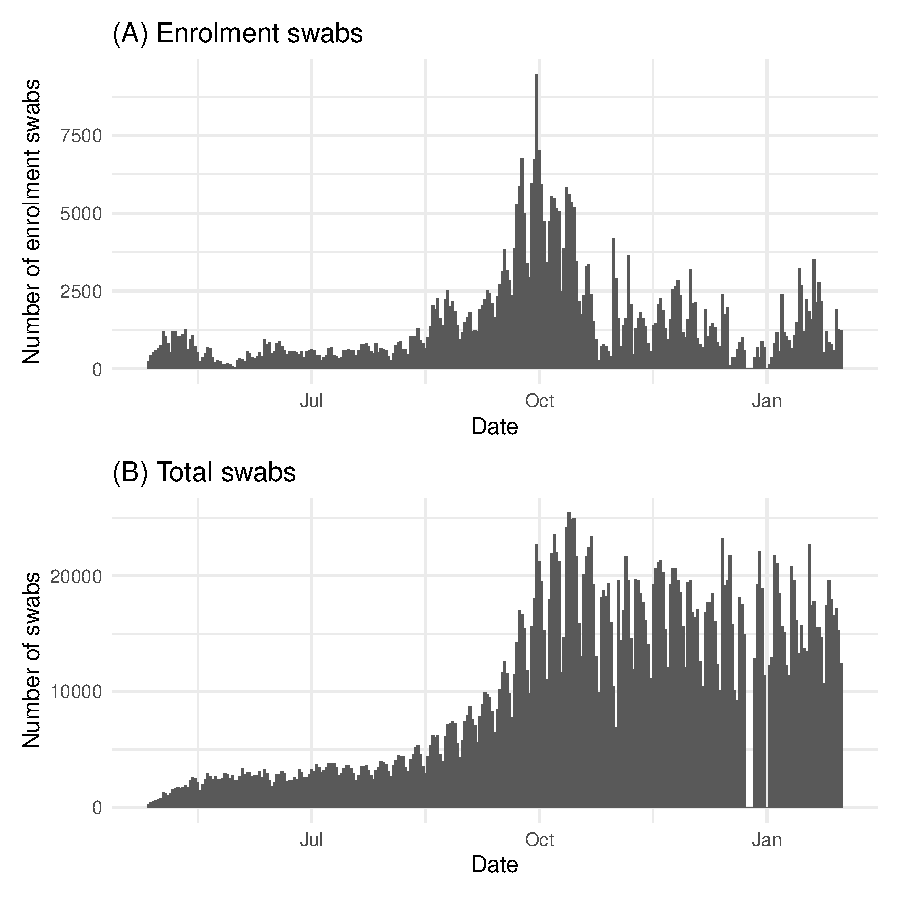
\includegraphics{biology-data/CIS-recruitment}
  \caption[CIS swab numbers]{%
    Number of swabs taken by the CIS in the period considered in this thesis (Sep 2020 until Jan 2021).
    (A) Only enrolment (\ie first) swabs for each individual.
    (B) Total swabs.
    Note the differing y-axis scales.
    Data from \textcite{CIStechData}.
  }
  \label{biology-data:fig:CIS-recruitment}
\end{figure}


\begin{figure}
  \centering 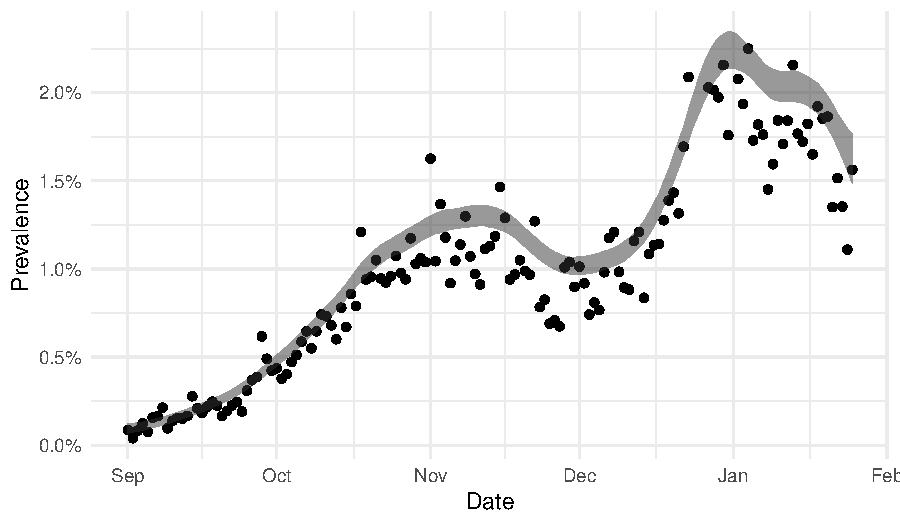
\includegraphics[width=\textwidth]{biology-data/CIS-positivity}
  \caption[CIS prevalence]{%
    CIS prevalence in the period considered in this thesis (Sep 2020 until Jan 2021).
    Dots show raw proportion of non-void tests that are positive on each day (days with fewer than 100 tests excluded for readability).
    Ribbon shows modelled 95\% CrI for the prevalence, corrected for non-response bias and smoothed over time (using the methodology described in \cref{E-backcalc:sec:methods}).
    The correction tends to increase the estimated prevalence because underrepresented groups tend to have higher prevalence.
  }
  \label{biology-data:fig:CIS-positivity}
\end{figure}
\begin{figure}
  \centering 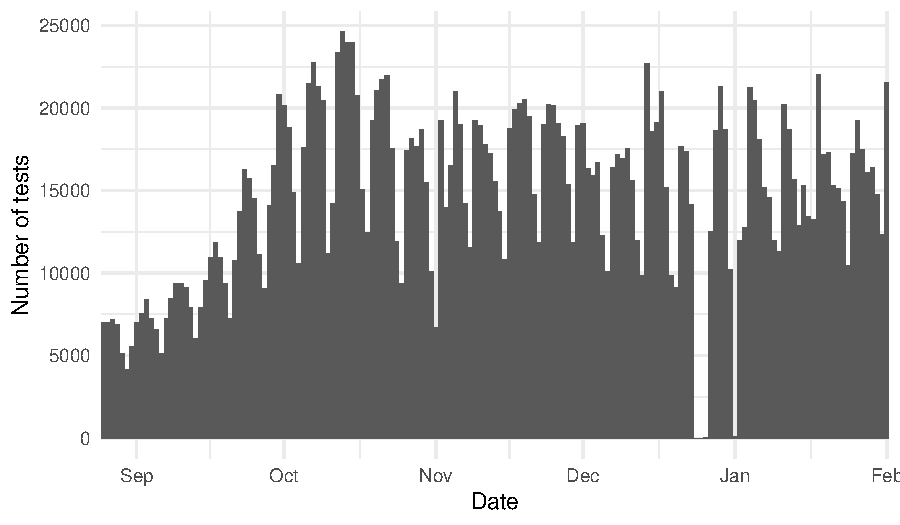
\includegraphics[width=\textwidth]{biology-data/CIS-num-tests}
  \caption[Number of CIS tests]{%
    Daily number of CIS tests conducted in the period considered in this thesis (Sep 2020 until Jan 2021).
  }
  \label{biology-data:fig:CIS-num-tests}
  \todo[inline]{Cut this repetition of number of tests? Maybe highlight period of interest in previous plot}
\end{figure}

\subsubsection{Episodes}

For the work in \cref{E-cis-perf-testing,E-cis-imperf-testing}, positive test results need to be grouped into \emph{infection episodes}.
An infection episode is a series of positive tests that are part of the same infection.
I use a method developed throughout the pandemic, and published within \textcite{weiRisk}; see that publication for full justification of the criteria.
Denote the time of a positive test by $t$, the number of consecutive negative tests prior to $t$ by $n$, and the time of the first positive test in the same individual by $t_p$ ($t_p = -\infty$ if there is no previous positive test in the same individual).
The test at $t$, in the pre-Omicron era (prior to December 2021), is defined as the start of a new infection episode if any of the following apply.
\begin{enumerate}
  \item $t_p = -\infty$.
  \item $n \geq 1$ and $t - t_p > 120$.
  \item $n \geq 2$ and $t - t_p > 90$.
  \item $n \geq 3$ and $t - t_p > 60$.
  \item $n \geq 4$.
  \item A complex heuristic based on the likely variant of the positive tests (see \textcite{weiRisk} for details). This heuristic rarely applied in the pre-Omicron era~\citePersonalComms{Sarah Walker}.
\end{enumerate}

A negative between two positive tests, when those positives are classed as part of the same infection episode, is known as an \emph{intermittent negative}.
Intermittent negatives are the clearest example of a false negative.
An intermittent negative is when an individual tests negative but tested positive previously and subsequently.
Intermittent negatives are stripped out when creating the dataset used for all duration analyses in this chapter, but demonstrate that false negatives do occur.

% Whether a future positive is part of the same episode of a reinfection is not always trivial; I rely on a process developed previously by Sarah Walker, see \cref{E-episode-def}.


\ifSubfilesClassLoaded{
  \listoftodos
}{}

\end{document}